\documentclass[12pt,a4paper]{article}
\usepackage[utf8]{inputenc}
\usepackage[spanish]{babel}
\usepackage{amsmath}
\usepackage{amsfonts}
\usepackage{amssymb}
\usepackage{graphicx}
\usepackage[left=2cm,right=2cm,top=2cm,bottom=2cm]{geometry}

\usepackage{enumitem}
\usepackage{algorithm}
\usepackage{algorithmic}
\usepackage[hidelinks]{hyperref}

\usepackage{subcaption}
\usepackage{pgfplots}

% Para la tabla
\usepackage[normalem]{ulem}
\useunder{\uline}{\ul}{}


\author{Ignacio Aguilera Martos}
\title{Práctica 2 \\ Aprendizaje Automático}
\date{22 de Abril de 2019}

\setlength{\parindent}{0cm}
\setlength{\parskip}{10px}


\begin{document}
	\maketitle

	\tableofcontents

	\newpage

\section{Ejercicio 1}

\subsection{Apartado 1}

Dibujemos en primer lugar la gráfica que se nos pide tanto con una uniforme como con una distribución normal o gaussiana.

\begin{figure}[H]
	\centering
	\begin{subfigure}{0.47\textwidth}
		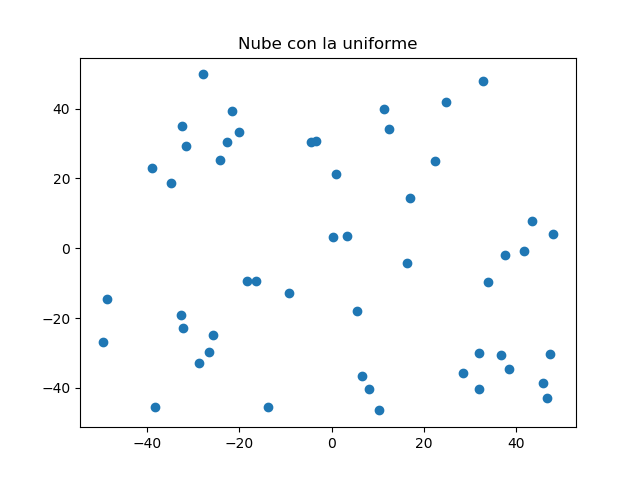
\includegraphics[scale=0.55]{./Imagenes/ej1-1.png}
		\caption{Nube generada con una uniforme}
	\end{subfigure}
	\begin{subfigure}{0.47\textwidth}
		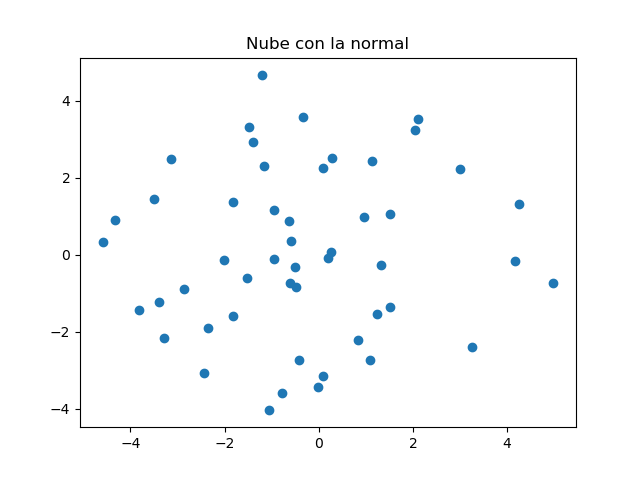
\includegraphics[scale=0.55]{./Imagenes/ej1-2.png}
		\caption{Nube generada con una normal}
	\end{subfigure}
\end{figure}

Podemos observar que el comportamiento de generación de puntos es completamente distinto. En el caso de la uniforme los puntos se generan de forma aleatoria de forma que la probabilidad de sacar un punto es la misma para todos los del cuadrado. Esto es, en la generación de datos el punto $(-40,40)$ y $(20,16)$ tienen la misma probabilidad de ser elegidos. Esto no es así en el caso de la normal. En este caso la probabilidad de escoger un punto es mayor a medida que nos acercamos al centro del cuadrado. Es por esto que podemos ver una concentración de los puntos en el centro y no en las esquinas.

\subsection{Apartado 2}

Tal y como dice el enunciado vamos a tomar la función $f(x,y) = y-ax-b$ siendo $a,b$ los parámetros de una recta generada de forma aleatoria por las funciones dadas en la plantilla. Vamos a separar la nube de puntos, esto es asignar etiquetas en función del signo de esta función.

Veamos el resultado:

\begin{figure}[H]
	\centering
	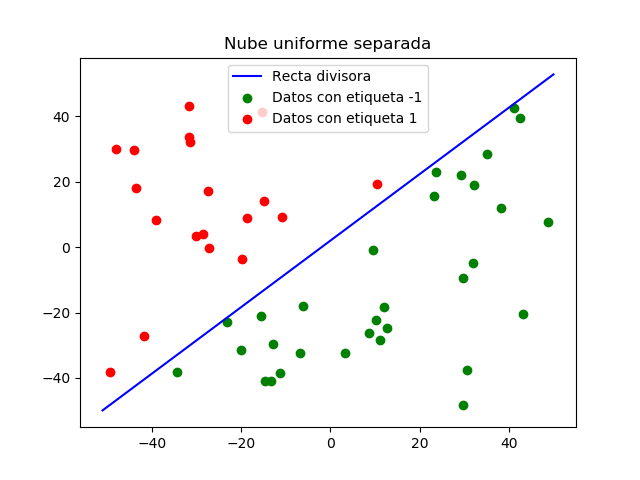
\includegraphics[scale=0.8]{./Imagenes/ej1-3.png}
	\caption{Nube separada de forma correcta}
\end{figure}

Tras esto se nos pide que induzcamos un 10\% de ruido en el conjunto de datos, esto es cambiar la etiqueta por la opuesta en un 10\% de los datos y que veamos que ahora hay puntos mal clasificados.

\begin{figure}[H]
	\centering
	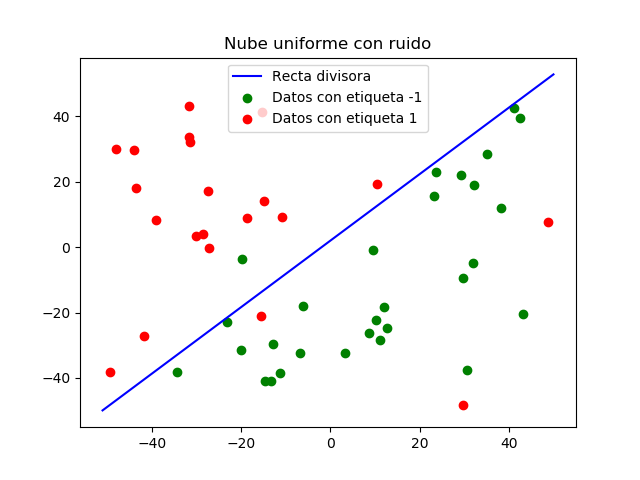
\includegraphics[scale=0.8]{./Imagenes/ej1-4.png}
	\caption{Nube separada de forma incorrecta}
\end{figure}

Como podemos observar ahora tenemos puntos mal clasificados a ambos lados de la recta.

Ahora el enunciado nos propone la utilización de funciones más sofisticadas para la división de nuestros datos, observemos los resultados:

\begin{figure}[H]
	\centering
	\begin{subfigure}{0.49\textwidth}
		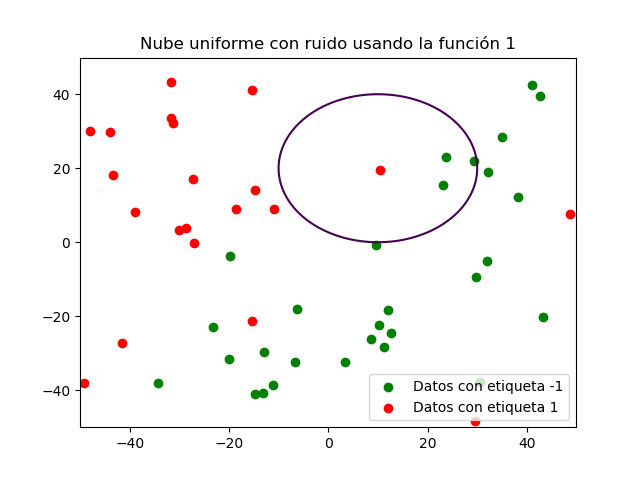
\includegraphics[scale=0.55]{./Imagenes/ej1-5.png}
		\caption{$f(x,y) = (x-10)^2 + (y-20)^2 - 400$}
	\end{subfigure}
	\begin{subfigure}{0.49\textwidth}
		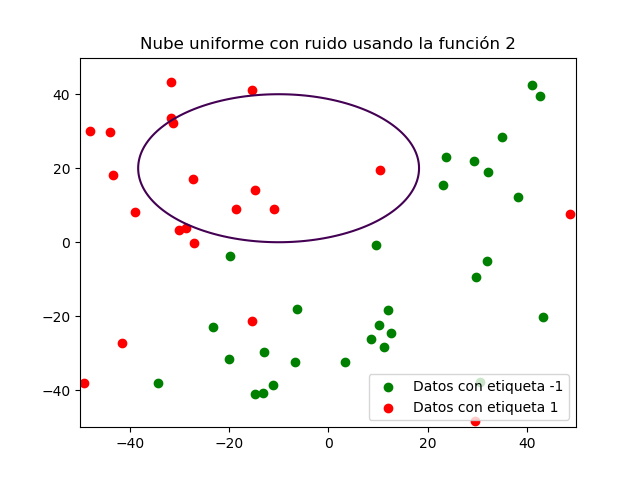
\includegraphics[scale=0.55]{./Imagenes/ej1-6.png}
		\caption{$f(x,y) = 0.5(x+10)^2 + (y-20)^2 - 400$}
	\end{subfigure}
\end{figure}

\begin{figure}[H]
	\centering
	\begin{subfigure}{0.49\textwidth}
		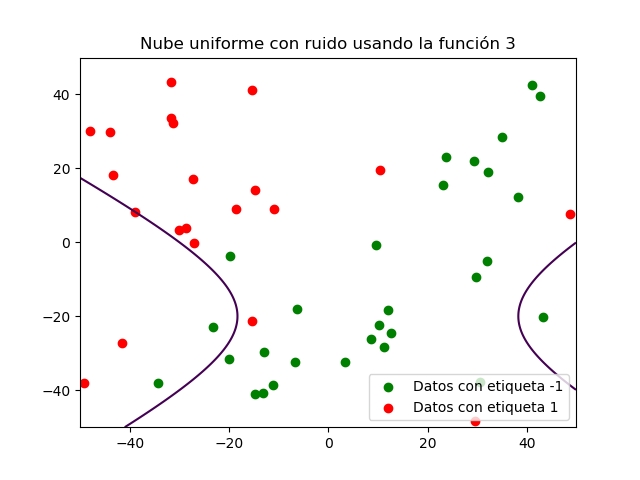
\includegraphics[scale=0.55]{./Imagenes/ej1-7.png}
		\caption{$f(x,y) = 0.5(x-10)^2 + (y+20)^2 - 400$}
	\end{subfigure}
	\begin{subfigure}{0.49\textwidth}
		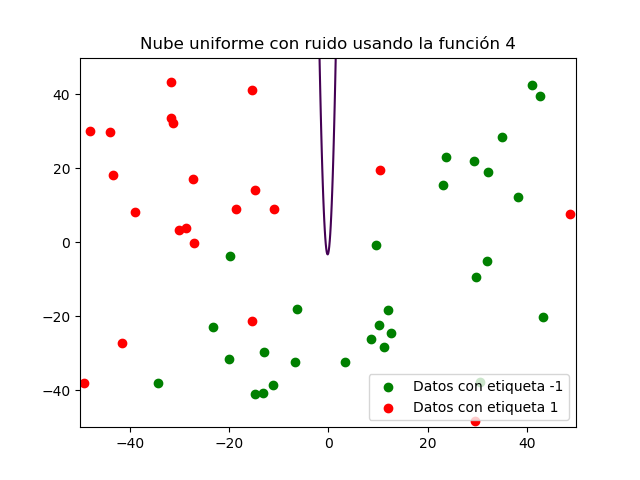
\includegraphics[scale=0.55]{./Imagenes/ej1-8.png}
		\caption{$f(x,y) = y-20x^2-5x+3$}
	\end{subfigure}
\end{figure}

Como podemos observar estas funciones son más sofisticadas que una línea. Las regiones obtenidas son mucho peores que las obtenidas por la recta original, pues los datos iniciales son datos que están muy cerca de ser separables y por tanto divisibles mediante una recta como frontera. Es por esto que en este tipo de casos en los que los datos son separables o muy cercanos a serlos las funciones más complejas o de mayor orden no nos aportan una ventaja con respecto a las lineales.

Si tuviéramos que extraer una ventaja de este tipo de funciones es la versatilidad que tienen pues, con coeficientes adecuados pueden obtenerse funciones tanto lineales como de orden superior, por ejemplo si tuviéramos en la función 4 los parámetros $f(x,y) = ay-bx^2 - cx + d$ tomando $b=0$ obtendríamos una función de tipo lineal, por lo tanto con este tipo de funciones abarcaríamos los casos lineales y casos cuadráticos en un eje.

Por tanto y como conclusión final, estas nuevas funciones no representan una mejoría con respecto a la función lineal debido a que los datos originales eran separables o muy cercanos a serlo y en estos casos las funciones lineales dan mejores resultados.

\section{Ejercicio 2}

\subsection{Apartado 1}

En este apartado lo primero que se nos pide es implementar el algoritmo Perceptrón. Este algoritmo discurre de la siguiente forma:

En primer lugar partimos de un valor inicial de w. Para cada dato y etiqueta verdadera de dicho dato comprobamos si la clasificación que nuestro w da para dicho dato es correcta. En caso de no serlo aplicamos una corrección de w en el sentido correcto, esto es, actualizamos w sumando el dato por su etiqueta. De esta forma garantizamos que en la siguiente iteración o lo clasificamos bien o estamos más cerca de hacerlo. El algoritmo se repite hasta que se agoten el número de iteraciones o bien no se modifique w en una pasada completa por el conjunto de datos.

Vamos a observar en primer lugar el comportamiento partiendo del w inicial $w=(0,0,0)$:

\begin{figure}[H]
	\centering
	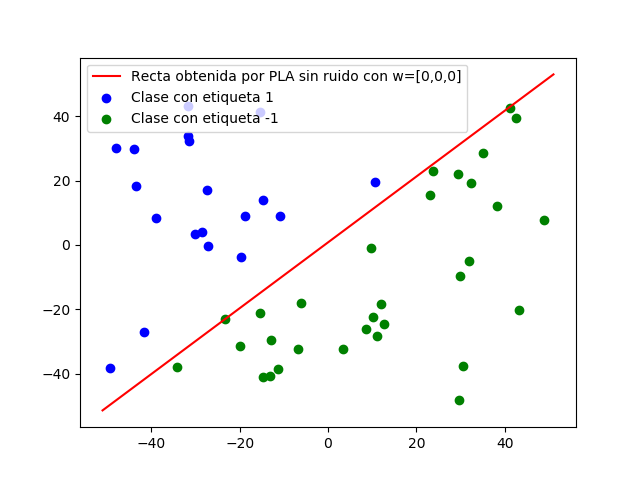
\includegraphics[scale=0.8]{./Imagenes/ej2-1.png}
	\caption{Resultados obtenidos con $w_{ini}=(0,0,0)$}
\end{figure}

El algoritmo en este caso ha convergido en 40 iteraciones. El simple hecho de haber convergido significa que la clasificación es perfecta, pues sólo para cuando ha dado una pasada completa al dataset y todos los datos estaban bien clasificados.

El enunciado tras esto nos pide que obtengamos valores de w iniciales de forma aleatoria, veamos cómo se comporta el algoritmo empezando en un punto aleatorio:

\begin{figure}[H]
	\centering
	\begin{subfigure}{0.32\textwidth}
		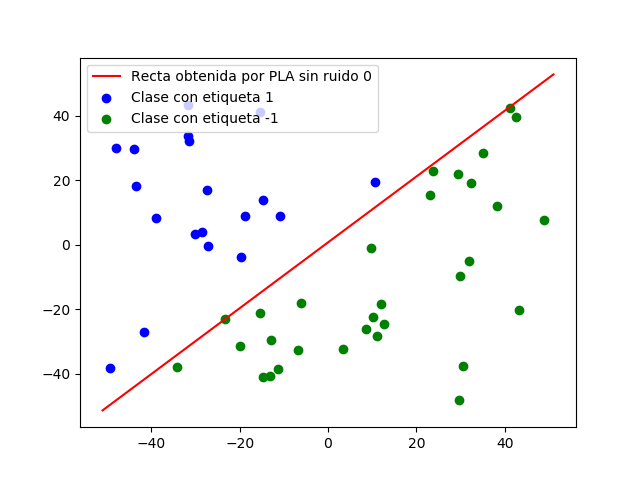
\includegraphics[scale=0.37]{./Imagenes/ej2-2.png}
		\caption{$w_{ini} = (0.877,0.188,0.062)$}
	\end{subfigure}
	\begin{subfigure}{0.33\textwidth}
		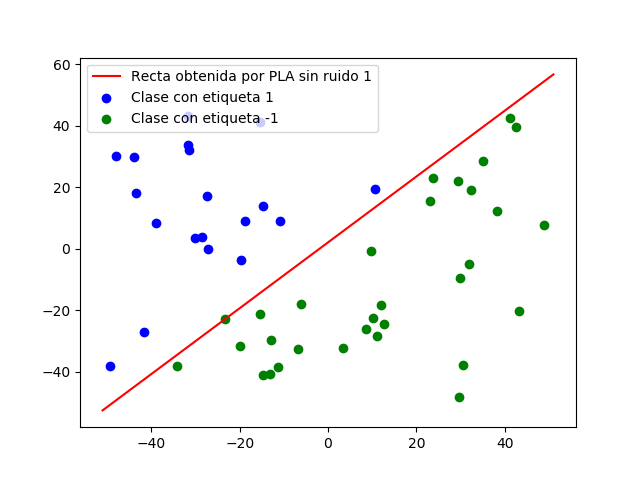
\includegraphics[scale=0.37]{./Imagenes/ej2-3.png}
		\caption{$w_{ini} = (0.927,0.814,0.217)$}
	\end{subfigure}
	\begin{subfigure}{0.33\textwidth}
		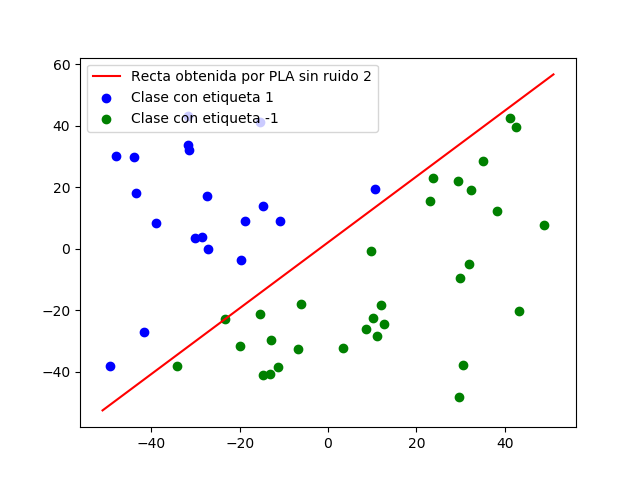
\includegraphics[scale=0.37]{./Imagenes/ej2-4.png}
		\caption{$w_{ini} = (0.050,0.577,0.467)$}
	\end{subfigure}
\end{figure}

\begin{figure}[H]
	\centering
	\begin{subfigure}{0.32\textwidth}
		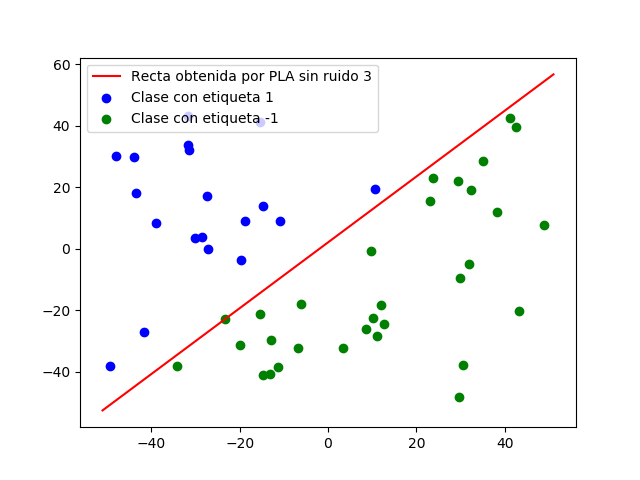
\includegraphics[scale=0.37]{./Imagenes/ej2-5.png}
		\caption{$w_{ini} = (0.357,0.424,0.305)$}
	\end{subfigure}
	\begin{subfigure}{0.33\textwidth}
		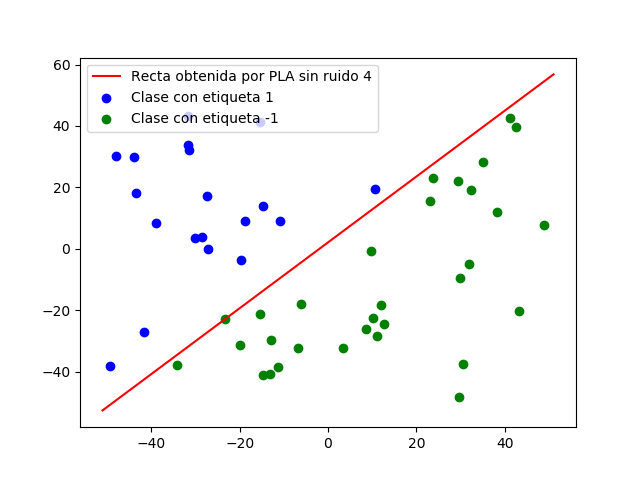
\includegraphics[scale=0.37]{./Imagenes/ej2-6.png}
		\caption{$w_{ini} = (0.412,0.312,0.808)$}
	\end{subfigure}
	\begin{subfigure}{0.33\textwidth}
		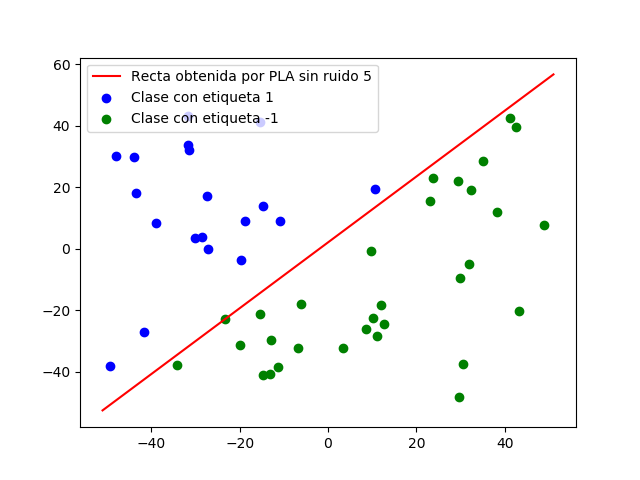
\includegraphics[scale=0.37]{./Imagenes/ej2-7.png}
		\caption{$w_{ini} = (0.672,0.327,0.811)$}
	\end{subfigure}
\end{figure}

\begin{figure}[H]
	\centering
	\begin{subfigure}{0.32\textwidth}
		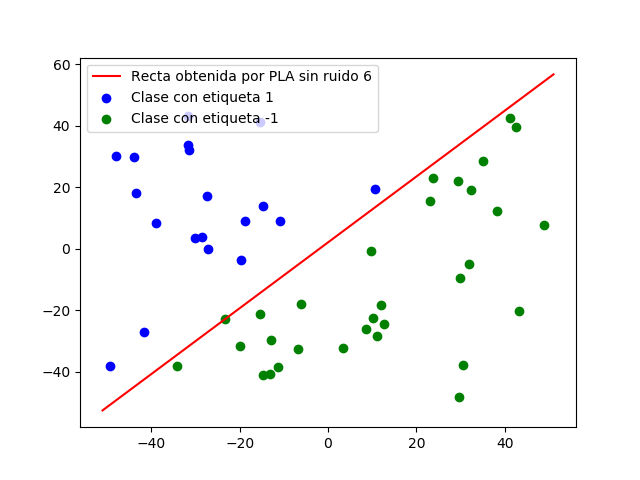
\includegraphics[scale=0.37]{./Imagenes/ej2-8.png}
		\caption{$w_{ini} = (0.484,0.641,0.395)$}
	\end{subfigure}
	\begin{subfigure}{0.33\textwidth}
		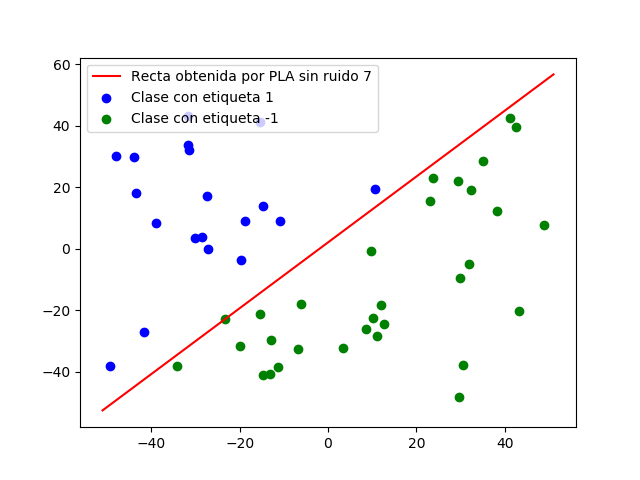
\includegraphics[scale=0.37]{./Imagenes/ej2-9.png}
		\caption{$w_{ini} = (0.036,0.552,0.524)$}
	\end{subfigure}
	\begin{subfigure}{0.33\textwidth}
		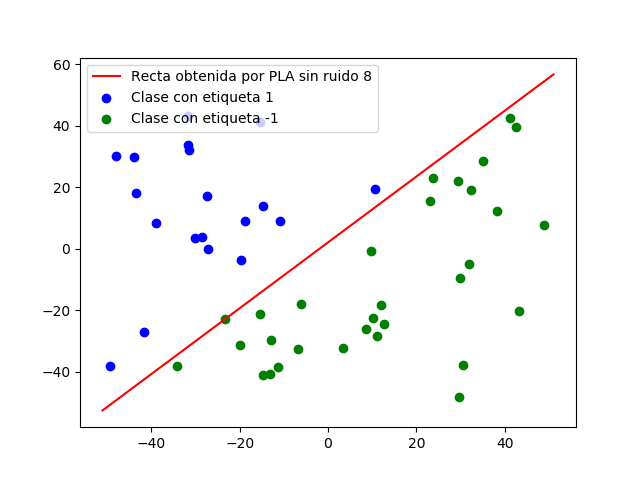
\includegraphics[scale=0.37]{./Imagenes/ej2-10.png}
		\caption{$w_{ini} = (0.770,0.764,0.217)$}
	\end{subfigure}
\end{figure}

\begin{figure}[H]
	\centering
	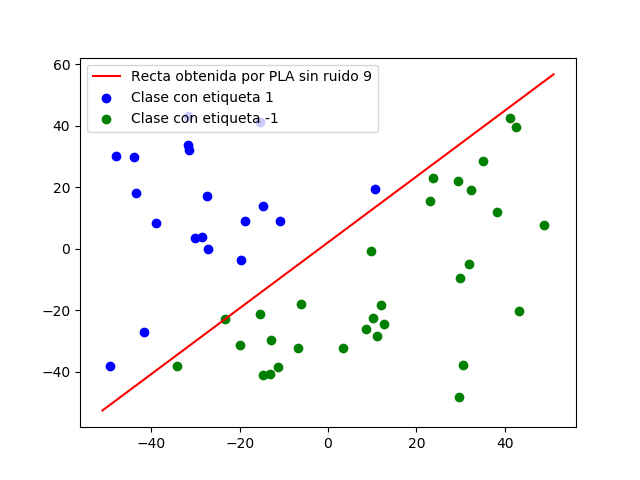
\includegraphics[scale=0.37]{./Imagenes/ej2-11.png}
	\caption{$w_{ini} = (0.601,0.432,0.335)$}
\end{figure}

Como podemos observar las 10 iteraciones han convergido de forma exitosa y lo han hecho empleando los siguientes números de iteraciones: $40$,$179$,$179$,$179$,$180$,$180$,$179$,$179$,$179$ y $179$ de donde podemos obtener que el número medio de iteraciones empleado ha sido de $165,3$ iteraciones.

Como podemos observar las mejores ejecuciones han sido las que partían de $(0,0,0)$ y la primera aleatoria que han conseguido clasificar todo el dataset de forma correcta en tan solo 40 iteraciones. El resto han necesito 179 o 180 iteraciones para conseguir el mismo resultado. Esto nos puede indicar que el w objetivo está cercano al $(0,0,0)$ o al menos más cercano que el resto de los w iniciales aleatorios que he generado. Aún así la convergencia ha sido rápida (aunque el número de datos no era muy grande) para este conjunto de datos concreto. Podemos ver por tanto en la diferencia de iteraciones dependiendo del punto inicial escogido que este hecho es muy determinante, por tanto escoger un w inicial adecuado hace que el algoritmo converja mucho más rápido que si lo escogemos en general de forma aleatoria.

El siguiente apartado nos pide realizar este mismo experimento pero empleando el conjunto de datos con ruido del ejercicio anterior. Veamos los resultados:

\begin{figure}[H]
	\centering
	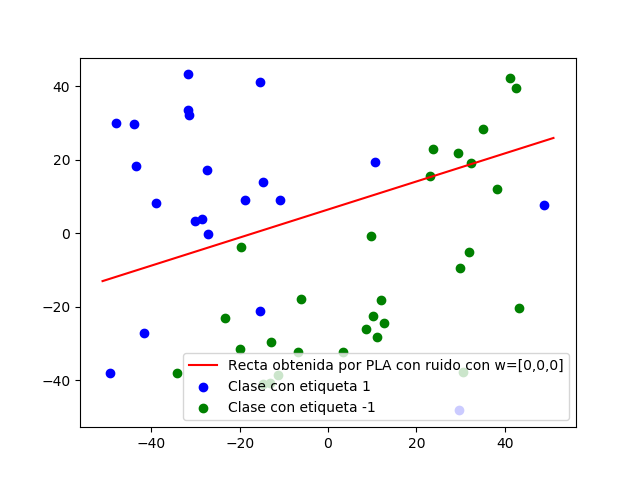
\includegraphics[scale=0.8]{./Imagenes/ej2-12.png}
	\caption{Resultados obtenidos con $w_{ini}=(0,0,0)$}
\end{figure}

Como podemos observar la clasificación no es correcta, es decir, no hemos obtenido una clasificación perfecta como se espera de este algoritmo. En este caso el problema es evidente y es que los datos no son separables. Esto implica que no existe una función lineal que divida perfectamente a los datos y por tanto no se produce la convergencia del algoritmo. En este algoritmo en concreto no sólo tenemos que la clasificación no es perfecta si no que además no tenemos garantía de que el w devuelto sea el mejor obtenido hasta el momento, es decir, el que menor error ha cometido a lo largo de la ejecución. Por tanto si este algoritmo no converge debemos pensar en emplear un algoritmo distinto o una modificación de PLA que mantenga el mejor resultado hasta el momento.

Por último cabe decir que como no se ha logrado clasificar perfectamente el dataset se ha agotado el número de iteraciones máximas establecidas, en este caso 10.000.

\begin{figure}[H]
	\centering
	\begin{subfigure}{0.32\textwidth}
		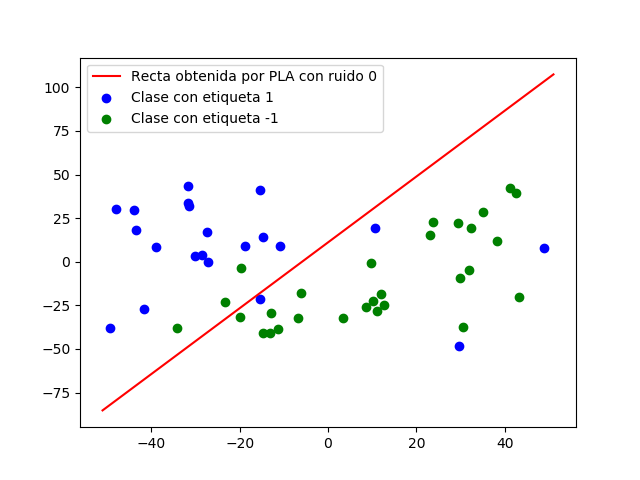
\includegraphics[scale=0.37]{./Imagenes/ej2-13.png}
		\caption{$w_{ini} = (0.396,0.299,0.375)$}
	\end{subfigure}
	\begin{subfigure}{0.33\textwidth}
		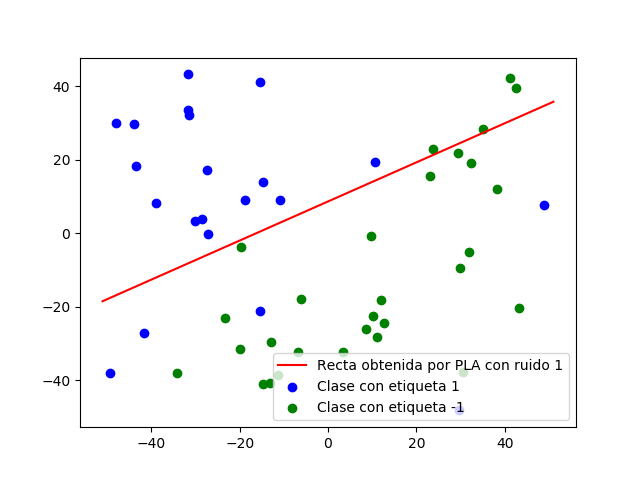
\includegraphics[scale=0.37]{./Imagenes/ej2-14.png}
		\caption{$w_{ini} = (0.659,0.136,0.633)$}
	\end{subfigure}
	\begin{subfigure}{0.33\textwidth}
		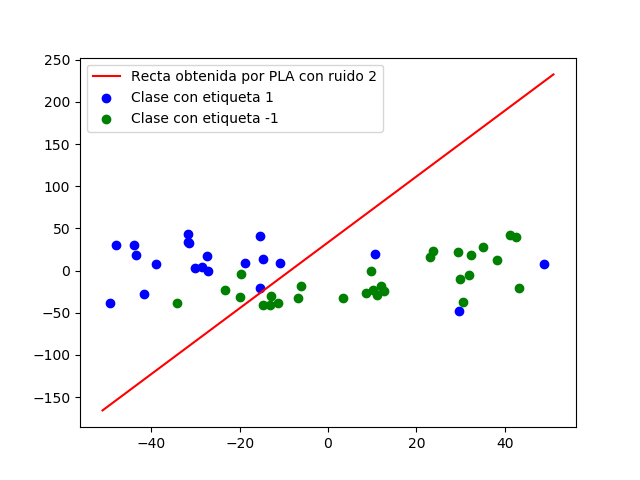
\includegraphics[scale=0.37]{./Imagenes/ej2-15.png}
		\caption{$w_{ini} = (0.087,0.956,0.693)$}
	\end{subfigure}
\end{figure}

\begin{figure}[H]
	\centering
	\begin{subfigure}{0.32\textwidth}
		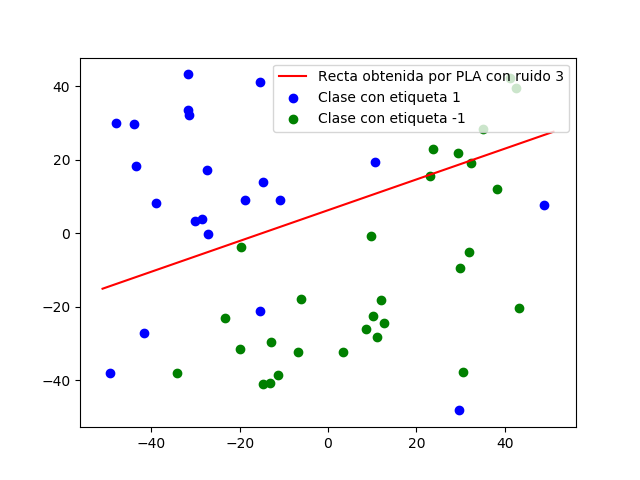
\includegraphics[scale=0.37]{./Imagenes/ej2-16.png}
		\caption{$w_{ini} = (0.408,0.651,0.300)$}
	\end{subfigure}
	\begin{subfigure}{0.33\textwidth}
		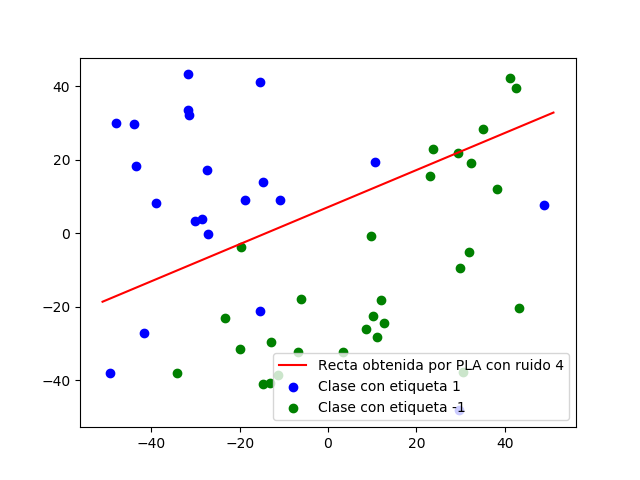
\includegraphics[scale=0.37]{./Imagenes/ej2-17.png}
		\caption{$w_{ini} = (0.105,0.528,0.528)$}
	\end{subfigure}
	\begin{subfigure}{0.33\textwidth}
		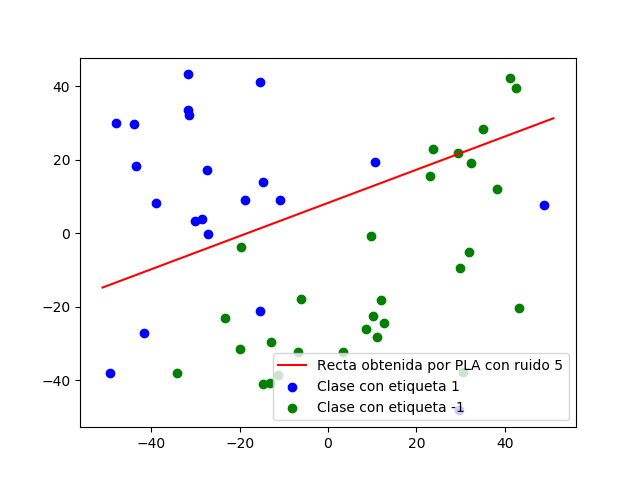
\includegraphics[scale=0.37]{./Imagenes/ej2-18.png}
		\caption{$w_{ini} = (0.602,0.005,0.838)$}
	\end{subfigure}
\end{figure}

\begin{figure}[H]
	\centering
	\begin{subfigure}{0.32\textwidth}
		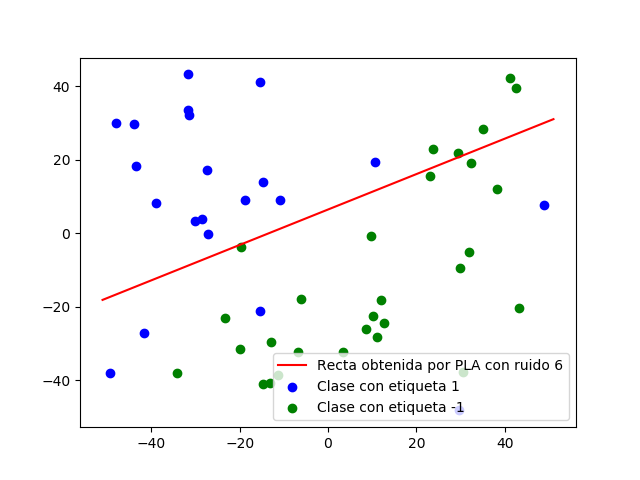
\includegraphics[scale=0.37]{./Imagenes/ej2-19.png}
		\caption{$w_{ini} = (0.482,0.893,0.152)$}
	\end{subfigure}
	\begin{subfigure}{0.33\textwidth}
		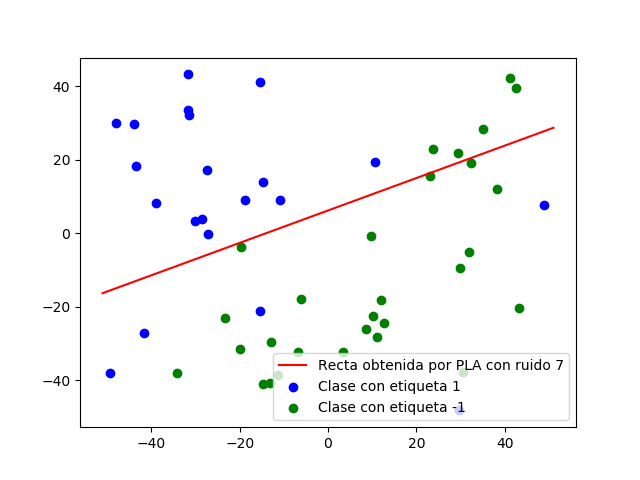
\includegraphics[scale=0.37]{./Imagenes/ej2-20.png}
		\caption{$w_{ini} = (0.761,0.575,0.059)$}
	\end{subfigure}
	\begin{subfigure}{0.33\textwidth}
		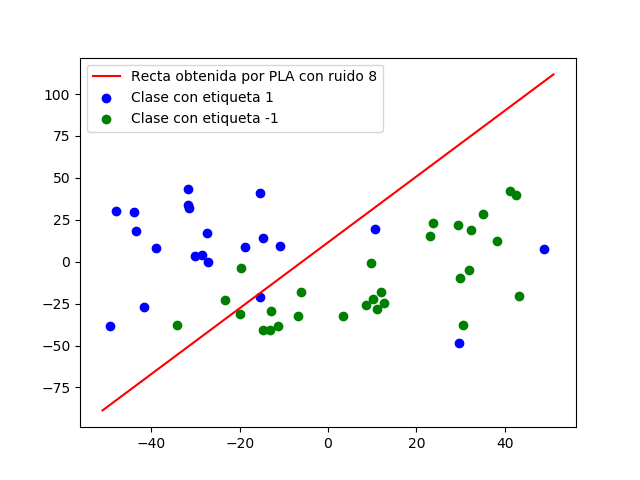
\includegraphics[scale=0.37]{./Imagenes/ej2-21.png}
		\caption{$w_{ini} = (0.823,0.407,0.246)$}
	\end{subfigure}
\end{figure}

\begin{figure}[H]
	\centering
	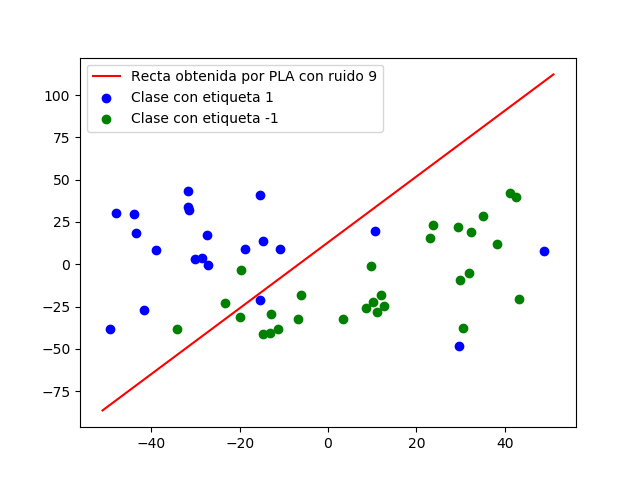
\includegraphics[scale=0.37]{./Imagenes/ej2-22.png}
	\caption{$w_{ini} = (0.591,0.095,0.902)$}
\end{figure}

La tendencia en todos los intentos es la misma pues el problema es el mismo. No se puede lograr la separación perfecta de los datos pues el conjunto no es separable, por lo que todos estos intentos han agotado las 10.000 iteraciones y no han conseguido clasificar perfectamente el conjunto de datos. Por ello el número medio de iteraciones consumidas es de 10.000 iteraciones.

\subsection{Apartado 2}

En este apartado se nos pide la implementación del algoritmo Gradiente Descendente Estocástico para Regresión Logística,veamos la implementación realizada de este algoritmo.

En primer lugar partimos de un vector $(0,0,0)$ como valor inicial. Mientras que la diferencia entre el w anterior y el w actual en norma sea mayor o igual que $0.01$ y no excedamos el número máximo de iteraciones entonces calculamos un conjunto de índices del conjunto de datos aleatorio y recorremos el dataset en ese orden aleatorio. Para cada dato actualizamos w con la fórmula:

$$w_{nuevo} = w_{antiguo}-\eta \frac{-y_n\cdot x_n}{1+e^{y_n w^T_{antiguo}x_n}}$$

Esta fórmula es el gradiente del error, que es $ln(1+e^{y_nw^Tx_n})$.

Usando esto lo que estamos haciendo es intentar minimizar el error de ajuste de la recta y por tanto intentar hallar una frontera adecuada de los datos. 

Además en este caso el algoritmo de gradiente descendente estocástico que estamos aplicando utiliza tamaño de minibatch 1.

El enunciado nos pide que generemos un conjunto de datos aleatorio mediante una uniforme y calculemos una recta aleatoria que hará de frontera entre las dos clases. Veamos el conjunto de datos obtenido:

\begin{figure}[H]
	\centering
	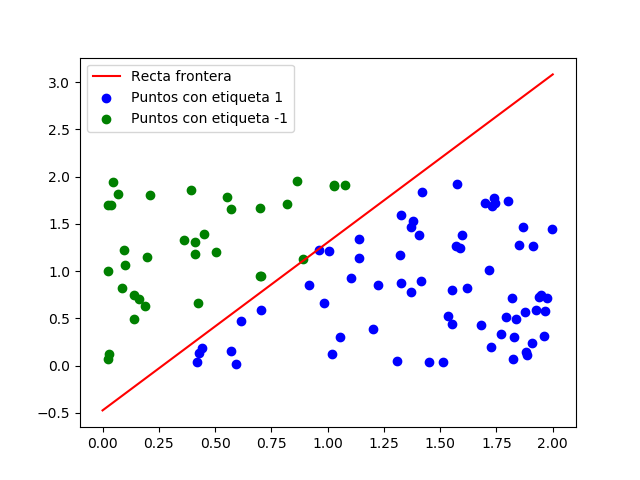
\includegraphics[scale=0.7]{./Imagenes/ej2-23.png}
	\caption{Conjunto de datos y frontera divisora}
\end{figure}

Veamos ahora el conjunto de datos y la recta obtenida mediante Gradiente Descendente Estocástico aplicado a Regresión Logística:

\begin{figure}[H]
	\centering
	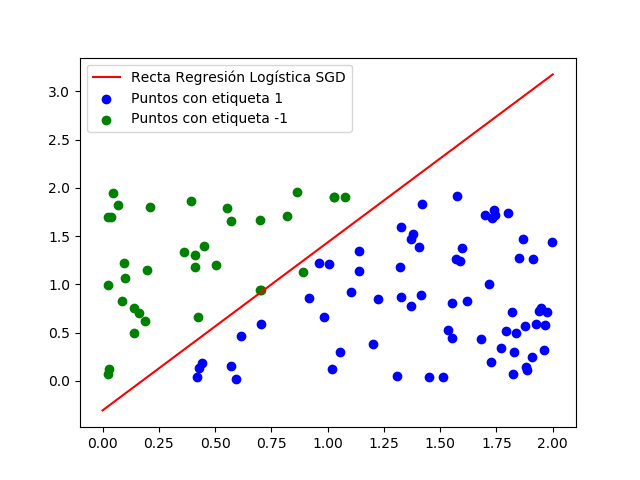
\includegraphics[scale=0.7]{./Imagenes/ej2-24.png}
	\caption{Conjunto de datos y frontera hallada por SGD aplicado a LR}
\end{figure}

El error cometido en esta aproximación ha sido de $E_{in}=0.0752599322594734$ y hemos tardado 311 iteraciones en conseguir el valor de $w$

Este error ha sido calculado utilizando que el error en cada punto se mide como $error_n(w) = \log (1+e^{-y_nw^Tx_n})$ de forma que el error que comete $w$ en todo el conjunto de datos es la media de los errores en cada punto.

En el segundo apartado se nos pide que una vez calculado este $w$ comprobemos cuál es el error si aumentamos el número de puntos de la nube uniforme calculada. Veamos las gráficas obtenidas y los errores:

\begin{figure}[H]
	\centering
	\begin{subfigure}{0.32\textwidth}
		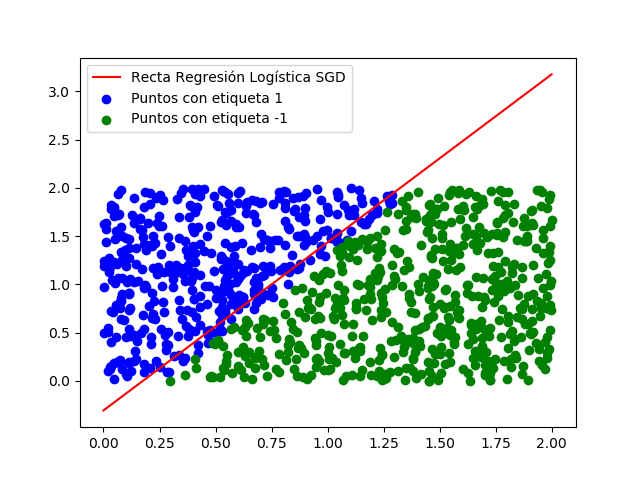
\includegraphics[scale=0.37]{./Imagenes/ej2-25.png}
		\caption{1.000 puntos}
	\end{subfigure}
	\begin{subfigure}{0.33\textwidth}
		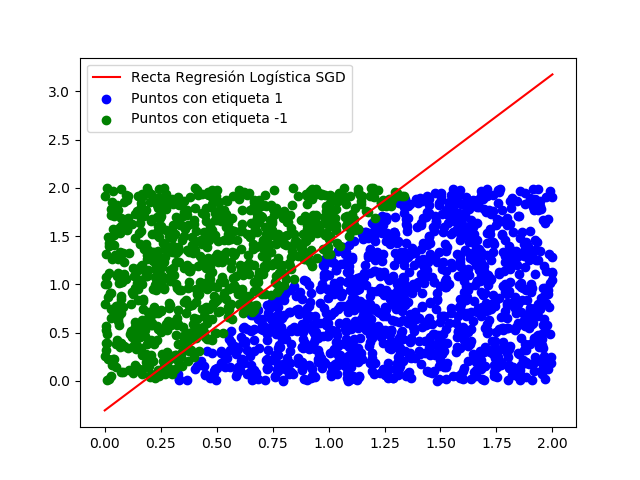
\includegraphics[scale=0.37]{./Imagenes/ej2-26.png}
		\caption{2.000 puntos}
	\end{subfigure}
	\begin{subfigure}{0.33\textwidth}
		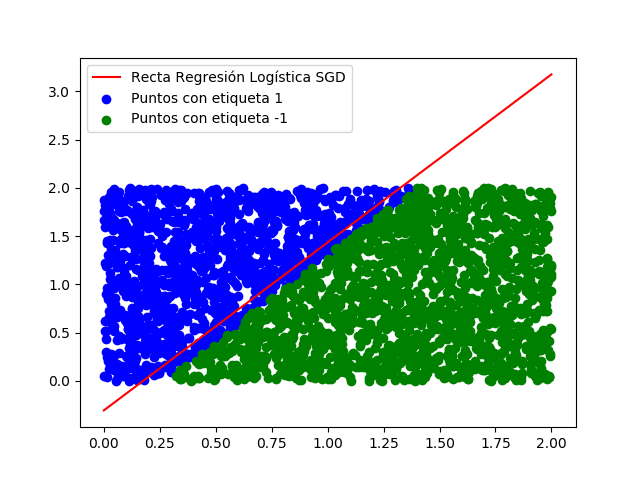
\includegraphics[scale=0.37]{./Imagenes/ej2-27.png}
		\caption{3.000 puntos}
	\end{subfigure}
\end{figure}

\begin{figure}[H]
	\centering
	\begin{subfigure}{0.44\textwidth}
		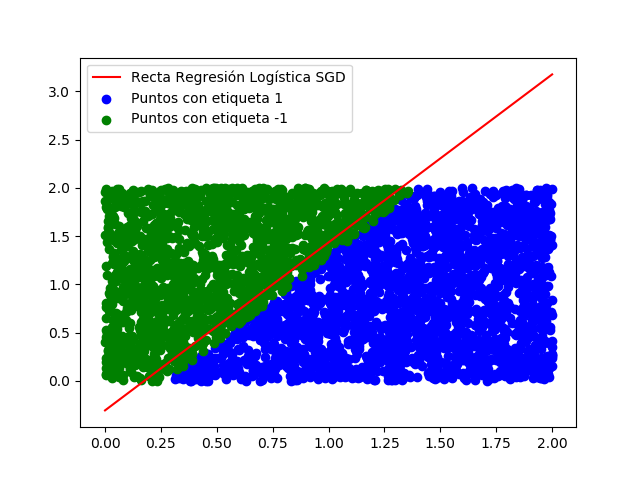
\includegraphics[scale=0.4]{./Imagenes/ej2-28.png}
		\caption{4.000 puntos}
	\end{subfigure}
	\begin{subfigure}{0.44\textwidth}
		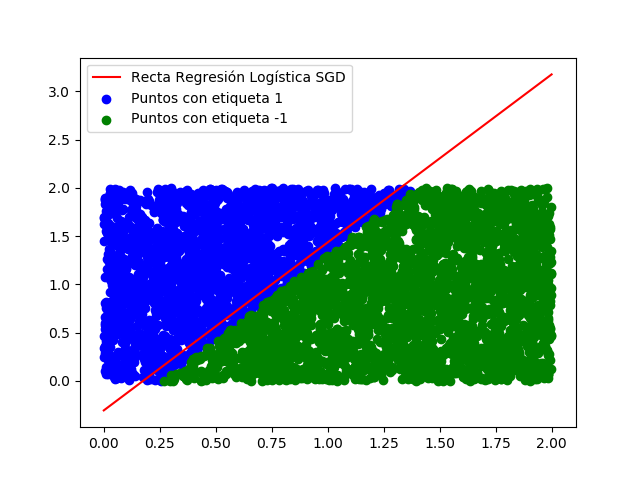
\includegraphics[scale=0.4]{./Imagenes/ej2-29.png}
		\caption{5.000 puntos}
	\end{subfigure}
\end{figure}

Como podemos observar la recta sigue clasificando los puntos de forma satisfactoria, al menos de forma visual. En estos casos con mayor número de puntos los errores cometidos han sido:

\begin{table}[H]
	\centering
	\begin{tabular}{|l|l|l|l|l|l|}
		\hline
		Número de puntos & 1000                & 2000                & 3000              & 4000                & 5000                \\ \hline
		$E_{out}$       & 0.12792 & 0.12064 & 0.12727 & 0.12414 & 0.11768 \\ \hline
	\end{tabular}
\end{table}

Podemos ver que el error dentro de la muestra es menor que el error fuera de la muestra para estos casos, pero además podemos apreciar una cierta tendencia a reducir el error a medida que aumentamos el número de puntos, cosa que ocurrirá hasta una cierta cota.

Como podemos observar la clasificación que hemos obtenido es buena en este caso.

\end{document}
